\documentclass[11pt]{article}
\usepackage{amsmath, amsthm, amssymb, pdfpages} 
\usepackage{fullpage}
\usepackage{hyperref}
\usepackage{graphicx}
\usepackage[capitalize]{cleveref}

% next three for UTF8 to work (for non-ASCII names to work without awkward codes)
\usepackage[T1]{fontenc}
\usepackage{textcomp}
\usepackage[utf8]{inputenc}

% import biblatex with prefered settings
% reuse code and library from LIGERA paper in the same repository
% loads biblatex with all the nice standard options that John determined some time ago!
% this version uses a ``Harvard'' style (first author last name, year in parentheses).
% also loads xpatch

% biblatex
% harvard style
\usepackage[style=authoryear,natbib,maxcitenames=2,doi=false,isbn=false,url=false,backend=bibtex]{biblatex}
% % numeric style
% \usepackage[style=numeric-comp,sorting=none,giveninits=true,doi=false,isbn=false,url=false,backend=bibtex]{biblatex}
% % to have citep etc work without a hitch here...
% \newcommand{\citep}{\cite}
% \newcommand{\citet}{\cite}

% remove "In: " before journal title
\renewbibmacro{in:}{}
% remove language
\AtEveryBibitem{\clearlist{language}}
% remove month
\AtEveryBibitem{\clearfield{month}}
% and also notes
\AtEveryBibitem{\clearfield{note}}
% remove dots between volume and issue
\usepackage{xpatch}
\xpatchbibmacro{volume+number+eid}{%
  \setunit*{\adddot}%
}{%
}{}{}
% put issue in parentheses
\DeclareFieldFormat[article]{number}{\mkbibparens{#1}}

\bibliography{../../manuscripts/zotero, ../../manuscripts/dummy} % biblatex wants this in the preamble...

\usepackage[noT]{kinshipsymbols}
% % copy of \Fst from package `kinshipsymbols`

% some more definitions
\newcommand{\kinMat}{%
  \ensuremath{%
    \mathbf{\Phi}
  }%
  \xspace%
}%
\newcommand{\kinMatStdLim}{%
  \ensuremath{%
    \mathbf{\hat{\Phi}}^\text{std-lim}
  }%
  \xspace%
}%

% for theorems!
\usepackage{amsthm}
%\newtheorem{thm}{Theorem}[section]
\newtheorem*{thm}{Theorem}
%\newtheorem{lem}[thm]{Lemma}
\newtheorem*{lem}{Lemma}
% \newtheorem{lemma}[theorem]{Lemma}

% % double line spacing (PLoS wants this)
% \usepackage{setspace}
% \doublespacing
% spacing smaller than double
\renewcommand{\baselinestretch}{1.2}

\title{\Large \textbf{The effect of population kinship estimation bias in heritability estimation and genetic association}}
\author{Zhuoran Hou$^1$, Alejandro Ochoa$^{1,2,*}$}
\date{}

\begin{document}
\maketitle

\noindent
$^1$ Department of Biostatistics and Bioinformatics, Duke University, Durham, NC 27705, USA \\
$^2$ Duke Center for Statistical Genetics and Genomics, Duke University, Durham, NC 27705, USA \\
$^*$ Corresponding author: \texttt{alejandro.ochoa@duke.edu}


\begin{abstract}
  Population kinship matrices are estimated for a variety of applications, including estimation of heritability and to control for population structure in genetic association studies.
  Recent work found that the most common family of kinship estimators can be severely biased.
  In this work, we investigate the effect of this kinship bias on the two downstream applications of heritability estimation and genetic association.
  We present a novel trait simulation strategy that accurately parametrizes heritability, even when utilizing real genotypes.
  Using these simulations, we find that heritability estimation becomes biased when using such biased kinship matrices.
  Remarkably however, this kinship bias does not affect genetic associations based on either Principal Components Analysis (PCA) or Linear Mixed-effects Models (LMM).
  Lastly, we explain our empirical observations using theory.
  In particular, the exact form of the bias of the standard kinship estimator is such that it is compensated for by fitting the intercept in both PCA and LMM approaches, which model population structure via covariates, suggesting that downstream applications without this precise arrangement will not be robust to this kinship bias.
\end{abstract}

% \clearpage

% \tableofcontents

\clearpage
	
\section{Introduction}

We previously found that the most common family of kinship estimators is biased \citep{ochoa_fst2}.

GCTA estimated the heritability of human height from population data \citep{yang_common_2010}.
GCTA is based on the biased kinship estimator \citep{yang_common_2010,yang_gcta:_2011}.


\section{Methods}

\subsection{Genetic model}

Suppose there are $m$ biallelic loci and $n$ diploid individuals.
The genotype \xij at a locus $i$ of individual $j$ is encoded as the number of reference alleles, for a preselected but otherwise arbitrary reference allele per locus.
These genotypes can be treated as random variables structured according to relatedness.
If \kt is the kinship coefficient of two individuals $j$ and $k$, and \pit is the ancestral allele frequency at locus $i$, then under the kinship model \citep{ochoa_fst1,ochoa_fst2} the expectation and covariance are given by
\begin{align*}
  \E[\mathbf{X}]
  =
    2 \mathbf{p} \mathbf{1}_n^\intercal
  ,
  \quad\quad
  \Cov(\mathbf{x}_i)
  =
    4 \pit (1-\pit) \kinMat
    ,
\end{align*}
where $\mathbf{x}_i$ is the length-$n$ column vector of genotypes at locus $i$, $\mathbf{X} = (\mathbf{x}_i^\intercal)$ is the complete $m \times n$ genotype matrix, $\kinMat = (\kt)$ is the $n \times n$ kinship matrix, $\mathbf{p} = (\pit)$ is a length-$m$ column vector of ancestral allele frequencies, $\mathbf{1}_n = (1)$ is a length-$n$ column vector where every element is 1, and the $\intercal$ superscript denotes matrix transposition.
Both kinship ($\kinMat$) and ancestral allele frequencies ($\mathbf{p}$) are parameters that depend on the choice of ancestral population, for which the Most Recent Common Ancestor (MRCA) population is the most sensible choice \citep{ochoa_fst1,ochoa_fst2}.
In this work, to simplify notation, we omit cumbersome notation that marks this dependence of parameters on the choice of ancestral population, not do we explicitly condition on the ancestral population when calculating expectations and covariances as done in previous work, although it is done implicitly.
This and later notation is summarized in \cref{tab:notation}.

\begin{table}[b!]
  \centering
  \caption{\textbf{Mathematical notation.}}
  \label{tab:notation}
  \begin{tabular}{lll}
    \hline
    Variable                     & Dimensions   & Description                  \\
    \hline
    $m$                          & $1$          & Number of loci               \\
    $n$                          & $1$          & Number of individuals        \\
    $i$                          & $1$          & Locus (variant) index        \\
    $j,k$                        & $1$          & Individual indexes           \\
    $\mu$                        & $1$          & Trait mean                   \\
    $\sigma^2$                   & $1$          & Trait variance scale         \\
    $h^2$                        & $1$          & (Narrow-sense) Heritability  \\
    $\mathbf{X} = (\xij)$        & $m \times n$ & Genotype matrix              \\
    $\mathbf{x}_i = (\xij)$      & $n \times 1$ & Genotype vector at locus $i$ \\
    $\mathbf{y}$                 & $n \times 1$ & Trait vetor                  \\
    $\alpha$                     & $1$          & Intercept                    \\
    $\mathbf{\beta} = (\beta_i)$ & $m \times 1$ & Effect size coefficients     \\
    $\mathbf{\epsilon}$          & $n \times 1$ & Non-genetic random effect    \\
    $\mathbf{p} = (\pit)$        & $m \times 1$ & Ancestral allele frequencies \\
    $\kinMat = (\kt)$      & $n \times n$ & Kinship matrix               \\
    $\mathbf{1}_n$               & $n \times 1$ & Vector of ones               \\
    $\mathbf{I}_n$               & $n \times n$ & Identity matrix              \\
    \hline
  \end{tabular}
\end{table}

The length-$n$ quantitative trait vector $\mathbf{y}$ for all individuals is assumed to follow a linear polygenic model,
\begin{equation}
  \label{eq:trait}
  \mathbf{y}
  =
  \mathbf{1}_n \alpha + \mathbf{X}^\intercal \mathbf{\beta}  + \mathbf{\epsilon},
\end{equation}
where $\alpha$ is the intercept coefficient, $\mathbf{\beta} = (\beta_i)$ is a length-$m$ column vector of effect size coefficients for each locus $i$ (which may be zero), and $\mathbf{\epsilon}$ is a length-$n$ column vector of non-genetic effects.
To analyze the covariance structure of the trait, we shall treat $\alpha$ and $\mathbf{\beta}$ are fixed parameters, while $\mathbf{X}$ and $\mathbf{\epsilon}$ are random.
The non-genetic effects are assumed to be independent with variance $(1-h^2) \sigma^2$ given by the total trait variance scale $\sigma^2$ and the narrow-sense heritability $h^2$:
\begin{align*}
  \E[\mathbf{\epsilon}]
  =
  \mathbf{0}_n
  ,
  \quad\quad
  \Cov(\mathbf{\epsilon})
  =
  (1-h^2) \sigma^2 \mathbf{I}_n
  ,
\end{align*}
where $\mathbf{0}_n$ is a length-$n$ column vector of zeroes.
The expectation of the trait is therefore
\begin{align*}
  \E[\mathbf{y}]
  = \alpha \mathbf{1}_n + \E \left[ \mathbf{X}^\intercal \right] \mathbf{\beta} + \E[\mathbf{\epsilon}]
  = \alpha \mathbf{1}_n + 2 \mathbf{1}_n \mathbf{p}^\intercal \mathbf{\beta}
  = \mu \mathbf{1}_n
  , \quad\quad \text{where} \quad\quad
  \mu 
  =
  \alpha + 2 \mathbf{p}^\intercal \mathbf{\beta}
  .
\end{align*}
The covariance matrix of the trait is
\begin{align*}
  \Cov(\mathbf{y})
  =
  \left( \sum_{i=1}^m \Cov(\mathbf{x}_i) \beta_i^2 \right) + \Cov(\mathbf{\epsilon})
  =
  \kinMat \left( \sum_{i=1}^m 4 \pit (1-\pit) \beta_i^2 \right) + (1-h^2) \sigma^2 \mathbf{I}_n
  .
\end{align*}
Therefore, we can write the covariance in terms of the heritability and the overall variance scale, in a formulation that matches previous work [TODO: add citations]:
\begin{align*}
  \Cov(\mathbf{y})
  =
  \sigma^2 \left( 2 h^2 \kinMat  + (1-h^2) \mathbf{I}_n \right)
  , \quad\quad \text{where} \quad\quad
  \sigma^2 h^2 
  = 
  \sum_{i=1}^m 2 \pit (1-\pit) \beta_i^2
  .
\end{align*}
Since the above expectation and covariance is conditioned on the choice of ancestral population, and given in terms of parameters that depend on it (\pit and $\kinMat$), then the parameters $\mu, \sigma^2, h^2$ are all also dependent on the choice of ancestral population.

The parametrization of our model is equivalent to setting separate absolute scales to the genetic and environment variance components, as $\sigma^2_G = \sigma^2 h^2$ and $\sigma^2_E = (1-h^2) \sigma^2$, respectively, which results in $\sigma^2_G + \sigma^2_E = \sigma^2$ and $\sigma^2_G / (\sigma^2_G + \sigma^2_E) = h^2$, as desired.

The factor of two in front of $\kinMat$ is traditionally there so that for an unstructured population
$2 \kinMat = \mathbf{I}_n$, in which case the trait covariance simplifies to
$\Cov(\mathbf{y}) = \sigma^2 \mathbf{I}_n$ for any value of $h^2$.
More broadly, the variance of the trait for any outbred individual is $\sigma^2$ under this parametrization.

\subsection{Trait simulation algorithm}

Suppose the genotype matrix $\mathbf{X}$ is available, and we have fixed values for the number of causal loci $m_1$, the trait mean, variance scale, and heritability ($\mu, \sigma^2, h^2$).
The goal is to choose the intercept $\alpha$ and draw random effect sizes $\mathbf{\beta}$ that result in the desired trait parameters.
First we randomly select $m_1$ loci to be causal, and subset the genotype matrix $\mathbf{X}$ and ancestral allele frequency vector $\mathbf{p}$ so that from this point on they contain only those causal loci (they now have dimensions $m_1 \times n$ and length $m_1$, respectively).

Below we divide the algorithm into two steps: (1) scaling the effect sizes, and (2) centering the trait.
Each step forks into two cases: whether the true ancestral allele frequencies $\mathbf{p}$ are known or not (the latter requires a known kinship matrix $\kinMat$).

\subsubsection{Scaling effect sizes}

The initial effect sizes $\beta_i$ are drawn independently from a standard normal distribution:
$$
\beta_i \sim \text{N}(0, 1).
$$

First we consider the simpler case of known ancestral allele frequencies $\mathbf{p} = (\pit)$.
The initial genetic variance scale is
$$
\sigma^2_0
=
\sum_{i=1}^{m_1} 2 \pit (1-\pit) \beta_i^2
.
$$
We obtain the desired variance by dividing each $\beta_i$ by $\sigma_0$ (which results in a variance of 1) and then multiply by $h \sigma$ (which results in the desired variance of $h^2 \sigma^2$).
Combining both steps, the update is
$$
\mathbf{\beta}
\leftarrow
\mathbf{\beta} \frac{ h \sigma }{\sigma_0}
.
$$

Now we consider the case of unknown ancestral allele frequencies but known kinship matrix.
First, sample estimates $\mathbf{\hat{p}} = (\pith)$ of the ancestral allele frequencies are constructed from the genotype data as
$$
\pith
=
\frac{1}{2n} \mathbf{1}_n^\intercal \mathbf{x}_i
.
$$
Although this estimator is unbiased ($\E[\mathbf{\hat{p}}] = \mathbf{p}$), the resulting variance estimates of interest $\pith \left( 1-\pith \right)$ are downwardly biased \citep{ochoa_fst2}:
$$
\E \left[ \pith \left( 1-\pith \right) \right]
=
\pit(1-\pit) (1 - \bar{\varphi})
,
$$
where $\bar{\varphi} = \frac{1}{n^2} \mathbf{1}_n^\intercal \kinMat \mathbf{1}_n$ is the mean kinship coefficient in the data.
Therefore the initial genetic variance scale, estimated as
$$
\hat{\sigma}^2_0
=
\sum_{i=1}^{m_1} 2 \pith (1-\pith) \beta_i^2
,
$$
has an expectation of
$$
\E \left[ \hat{\sigma}^2_0 \right]
=
\sigma^2_0 (1 - \bar{\varphi})
.
$$
Therefore, assuming that this additional factor $(1 - \bar{\varphi})$ is known, the update
$$
\mathbf{\beta}
\leftarrow
\mathbf{\beta} \frac{ h \sigma \sqrt{1-\bar{\varphi}} }{\hat{\sigma}_0}
$$
results in the desired variance.

\subsubsection{Centering the trait}

Here we consider the problem of selecting the intercept coefficient $\alpha$ that, together with the previous effect size coefficient vector $\mathbf{\beta}$, result in the desired trait mean $\mu$.

When ancestral allele frequencies are known, the trait can be centered precisely.
Given our model, we obtain the desired overall trait mean $\mu$ by choosing the intercept coefficient to be
$$
\alpha 
=
\mu - 2 \mathbf{p}^\intercal \mathbf{\beta}
.
$$

When ancestral allele frequencies are unknown, the solution is to choose the intercept coefficient
\begin{align*}
  \alpha 
  =
  \mu - 2 \hat{\bar{p}} \mathbf{1}_{m_1}^\intercal \mathbf{\beta}
  , \quad\quad
  \hat{\bar{p}}
  =
  \frac{1}{m_1} \mathbf{1}_{m_1}^\intercal \mathbf{\hat{p}}
  =
  \frac{1}{ 2 m_1 n } \mathbf{1}_{m_1}^\intercal \mathbf{X}^\intercal \mathbf{1}_n
  =
  \frac{1}{2} \bar{X}
  ,
\end{align*}
where $\mathbf{1}_{m_1}$ is a length-$m_1$ column vector of ones.
Note that this overal mean allele frequency $\hat{\bar{p}}$ is computed among causal loci only.
This works very well in practice since $\mathbf{\beta}$ is drawn randomly, so it is uncorrelated to $\mathbf{p}$ and therefore
$$
\frac{1}{m_1} \mathbf{p}^\intercal \mathbf{\beta}
=
\frac{1}{m_1} \sum_{i=1}^{m_1} \pit \beta_i
\approx
\left( \frac{1}{m_1} \sum_{i=1}^{m_1} \pit \right)
\left( \frac{1}{m_1} \sum_{i=1}^{m_1} \beta_i \right)
=
\frac{1}{m_1}
\bar{p}
\mathbf{1}_{m_1}^\intercal \mathbf{\beta}
$$
is a good approximation.

Now we discuss why the more obvious naive approach, which would be to center the trait using estimated ancestral allele frequencies as
$
\alpha 
=
\mu - 2 \mathbf{\hat{p}}^\intercal \mathbf{\beta}
,
$
does not work.
This approach is equivalent to centering genotypes at each locus as
$$
\mathbf{y} = \alpha \mathbf{1}_n + \sum_{i=1}^{m_1} (\mathbf{x}_i - 2 \pith \mathbf{1}_n) \beta_i + \mathbf{\epsilon}.
$$
However, this operation introduces a distortion in the covariance of the genotypes \citep{ochoa_fst2}: 
$$
\Cov \left( \mathbf{x}_i - 2 \pith \mathbf{1}_n \right)
=
\pit ( 1 - \pit ) \left( 
\kinMat 
+ \bar{\varphi} \mathbf{1}_n \mathbf{1}_n^\intercal 
- \mathbf{\varphi} \mathbf{1}_n^\intercal 
- \mathbf{1}_n \mathbf{\varphi}^\intercal 
\right),
$$
where $\bar{\varphi}$ is the overall mean kinship, as before, and $\mathbf{\varphi} = \frac{1}{n} \kinMat \mathbf{1}_n$ is a length-$n$ column vector of per-row mean kinship values.
These undesireable distortions propagate to the trait, which we confirmed in simulations (not shown).
%It is not clear how to correct these distortions after centering the trait as shown above.
Note that the intercept version we chose instead does not induce this genotype centering, which prevents the undesireable distortions in the trait covariance.

\subsection{Admixture simulation for genotype matrices}

TODO: describe the BNPSD simulation.

\subsection{Kinship estimation}

TODO: Present our popkin estimator, standard estimator (MOR and ROM versions), and GCTA estimator (like standard-MOR but with diff diagonal), with limits.

\subsection{Heritability and genetic association software}

TODO: state versions, download links, etc.

Outline:
\begin{itemize}
\item SOLAR-Eclipse (herit only) \citep{almasy_multipoint_1998}.
\item GCTA (both heritability and genetic association) \citep{yang_gcta:_2011}.
\item PCA: our optimized R implementation [TODO: cite Yao and Ochoa].  Genetic association only.
\end{itemize}

\section{Results}

\subsection{Empirical demonstration of biases in heritability estimation}

TODO: add results using SOLAR and GCTA, varying the input kinship matrices (estimates and limits from methods).

GCTA results:

Figure 1 shows the distribution of heritability estimated by GCTA with different input kinship matrices. From the figure, we can see that the performance of the default kinship matrix of GCTA is different from others. These using popkin and std lim kinship matrices perform most similar to the one using true kinship matrix.

\begin{figure}[bp!]
  \centering
  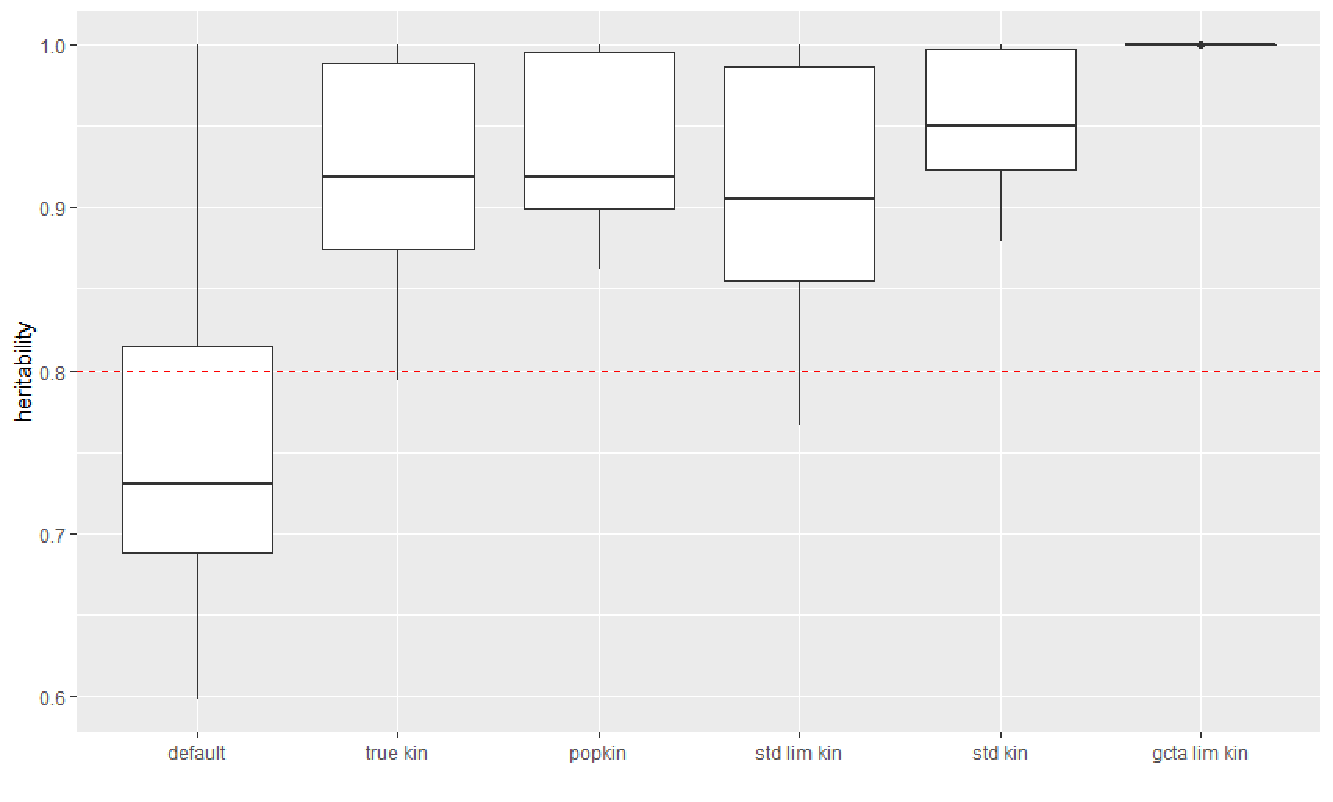
\includegraphics[width=6in]{herit_all_6_n_ind=2000-raw.pdf}
  \caption{
    {\bf Heritability estimation by GCTA with different kinship matrices.}
    $n_ind=2000 $ for 10 iteration, others are default settings ($m_loci= 100000$, $k_subpops=3$, $fst=0.3$, $bias_coeff=0.5$, $generations=1$, $herit=0.8$, $m_causal=100$).
  }
  \label{fig:heritability_estimation}
\end{figure}


\subsection{Empirical demonstration of robustness to kinship bias in PCA and LMM genetic assocation studies}

Figure 2 and 3 shows the correlation matrix of p-value and $\hat{\mathbf{\beta}}$ of PCA and GCTA (LMM based method) with different input kinship matrices. The figures show that all the methods are highly correlated, while results generated by LMM based methods tend to be more closely related.

\begin{figure}[bp!]
  \centering
  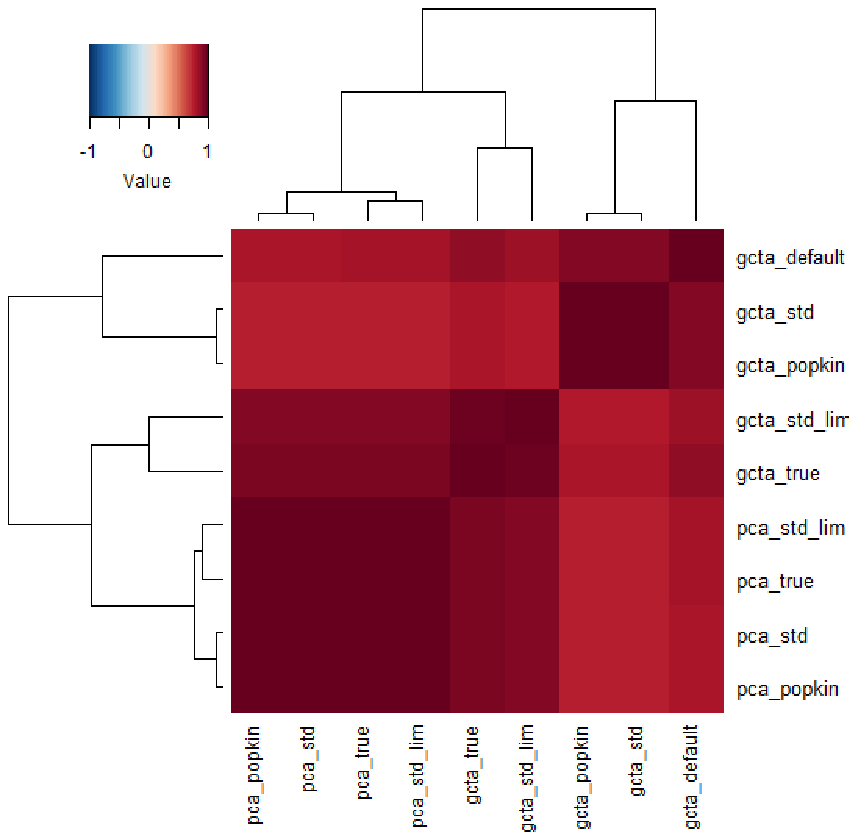
\includegraphics[width=6in]{all_pval.pdf}
  \caption{
    {\bf Heatmap and dendrogram for p-values of GCTA and PCA with different kinship matrices ($m=10,000$).}
    
  }
  \label{fig:all_pval}
\end{figure}

\begin{figure}[bp!]
  \centering
  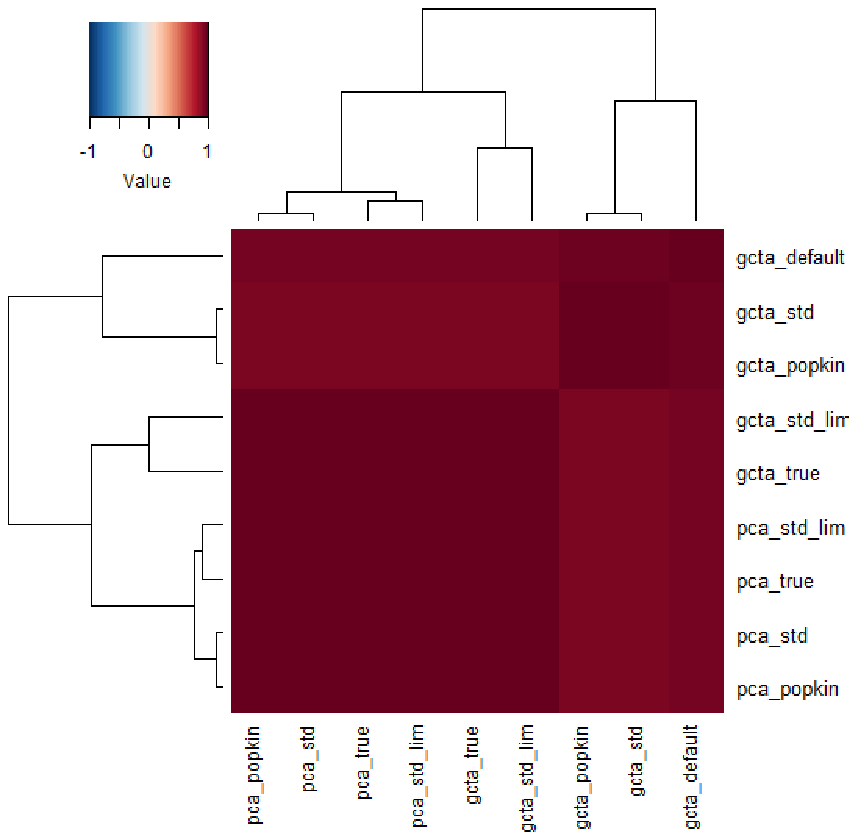
\includegraphics[width=6in]{all_beta_hat.pdf}
  \caption{
    {\bf Heatmap and dendrogram for $\hat{\mathbf{\beta}}$ of GCTA and PCA with different kinship matrices ($m=10,000$).}
  }
  \label{fig:all_beta_hat}
\end{figure}


\subsection{Theoretical justification of empirical observations}

Here, to eliminate random estimation noise from the analysis (which our empirical evaluations suggest play a minor role), we shall focus on the limiting bias of the standard kinship estimator.
Therefore, our theoretical results only consider the true kinship matrix \kinMat and the limit of the standard kinship estimator, given by
$$
\kinMatStdLim
=
\frac{1}{1 - \bar{\varphi}}
\left(
  \kinMat
  + \bar{\varphi} \mathbf{1}_n \mathbf{1}_n^\intercal 
  - \mathbf{\varphi} \mathbf{1}_n^\intercal 
  - \mathbf{1}_n \mathbf{\varphi}^\intercal 
\right)
.
$$
The two kinship matrices are related more succinctly using the centering matrix $\mathbf{C}$:
$$
\kinMatStdLim
=
\frac{1}{1 - \bar{\varphi}}
\mathbf{C} \kinMat \mathbf{C}
, \quad\quad
\mathbf{C}
=
\mathbf{I}_n - \frac{1}{n} \mathbf{1}_n \mathbf{1}_n^\intercal
.
$$

The centering matrix has been well studied, and we review its properties here.
For any length-$n$ vector $\mathbf{v}$ we have
\begin{align*}
  \mathbf{C} \mathbf{v}
  % =
  % \left(\mathbf{I} - \frac{1}{n} \mathbf{1} \mathbf{1}^\intercal\right) \mathbf{v}
  % =
  % \mathbf{I} \mathbf{v} - \frac{1}{n} \mathbf{1} \mathbf{1}^\intercal \mathbf{v}
  =
  \mathbf{v} - \mathbf{1}_n \bar{v}
  ,
\end{align*}
where $\bar{v} = \frac{1}{n} \mathbf{1}_n^\intercal \mathbf{v}$ is the mean value of the elements of $\mathbf{v}$.
Therefore, $\mathbf{v} = \mathbf{1}_n$ gets transformed to the zero vector, so it is an eigenvector with an eigenvalue of zero:
\begin{align*}
  \mathbf{C} \mathbf{1}_n
  % =
  % \mathbf{1} - \mathbf{1}
  =
  \mathbf{0}_n
  .
\end{align*}
Moreover, any vector $\mathbf{v}$ orthogonal to $\mathbf{1}_n$ has a zero mean element ($\bar{v} = 0$) by hypothesis and it is not altered by $\mathbf{C}$ ($\mathbf{C} \mathbf{v} = \mathbf{v}$).
Therefore, the nullspace of $\mathbf{C}$ is spanned by $\mathbf{1}_n$.

This centering matrix provides the key insight as to why PCA and LMM approaches are robust to this specific kinship bias, namely that by fitting the intercept term $\alpha \mathbf{1}_n$ together with the eigenvectors (for PCA) or random effects (in the same rowspace as the eigenvectors; for LMM) of \kinMatStdLim, they complete the rowspace of \kinMatStdLim to equal the rowspace of the true kinship matrix \kinMat plus the intercept.
First we show the following lemma.

\begin{lem}
  $\mathbf{1}_n$ is in the nullspace of \kinMatStdLim but not of \kinMat.
\end{lem}

\begin{proof}
The vector $\mathbf{1}_n$ is not in the nullspace of any true kinship matrix \kinMat, since $\kinMat \mathbf{1}_n \neq \mathbf{0}_n$, which follows since all kinship values are non-negative and the diagonal of the kinship matrix is strictly positive (it has a minimum value of $\frac{1}{2}$).
However, $\mathbf{1}_n$ is in the nullspace of \kinMatStdLim since $\mathbf{C} \mathbf{1}_n = \mathbf{0}_n$:
$$
\kinMatStdLim \mathbf{1}_n
=
\frac{1}{1 - \bar{\varphi}}
\mathbf{C} \kinMat \mathbf{C} \mathbf{1}_n
=
\mathbf{0}_n
.
$$
\end{proof}

Now we may prove the desired theorem.

\begin{thm}
  The rowspace of \kinMat and $\mathbf{1}_n$ equals rowspace of \kinMatStdLim and $\mathbf{1}_n$.
\end{thm}

\begin{proof}
  Since $\mathbf{1}_n$ is in both rowspaces, it suffices to consider vectors $\mathbf{v}$ orthogonal to $\mathbf{1}_n$, which satisfy $\mathbf{C} \mathbf{v} = \mathbf{v}$.
  We shall prove below that any such vector is in the nullspace of \kinMat if and only if it is in the nullspace of \kinMatStdLim.
  Then, since the nullspace of \kinMat and $\mathbf{1}_n$ is the same as the nullspace of \kinMatStdLim and $\mathbf{1}_n$, it follows from the fundamental theorem of linear algebra that their rowspaces are also the same.
  
  If $\mathbf{v}$ is in the nullspace of \kinMat, then $\kinMat \mathbf{v} = \mathbf{0}_n$.
  It follows that
  $$
  \kinMatStdLim \mathbf{v}
  =
  \frac{1}{1 - \bar{\varphi}}
  \mathbf{C} \kinMat \mathbf{C} \mathbf{v}
  =
  \frac{1}{1 - \bar{\varphi}}
  \mathbf{C} \kinMat \mathbf{v}
  =
  \mathbf{0}_n
  ,
  $$
  so $\mathbf{v}$ is also in the nullspace of \kinMatStdLim.
  
  Conversely, if $\mathbf{v}$ is in the nullspace of \kinMatStdLim, then $\kinMatStdLim \mathbf{v} = \mathbf{0}_n$, which implies that
  $
  \mathbf{C} \kinMat \mathbf{C} \mathbf{v}
  =
  \mathbf{C} \kinMat \mathbf{v}
  =
  \mathbf{0}_n
  $.
  Left multiplying by $\mathbf{v}^\intercal$ results in
  $
  \mathbf{v}^\intercal \mathbf{C} \kinMat \mathbf{v}
  =
  \mathbf{v}^\intercal \kinMat \mathbf{v}
  =
  0
  $, which implies that $\mathbf{v}$ is also in the nullspace of the positive-semidefinite matrix \kinMat, as desired.
  If \kinMat were positive definite, then no such $\mathbf{v} \ne \mathbf{0}_n$ would exist (\kinMat would have the trivial nullspace $\{ \mathbf{0}_n \}$).
\end{proof}

\subsubsection{Theoretical justification for PCA genetic association}

In PCA-based genetic association, the desired result follows from the previous theorem, as follows.
Here the goal is to fit the trait $\mathbf{y}$ using a model simiar to our main model in \cref{eq:trait}, namely
\begin{equation}
  \label{eq:pca_gwas}
  \mathbf{y}
  =
  \mathbf{1}_n \alpha + \mathbf{x}_i \beta_i + \mathbf{U}_r \mathbf{\gamma}_r + \mathbf{\epsilon}
  ,
\end{equation}
where instead of including the whole genotype matrix $\mathbf{X}$ as we did in \cref{eq:trait}, here the genotype vector $\mathbf{x}_i$ at a single locus $i$ is fit, and the effect of the rest of the genome is approxiated using the top $r$ eigenvectors of the kinship matrix, contained in the $n \times r$ matrix $\mathbf{U}_r$ and its length-$r$ vector of coefficients $\mathbf{\gamma}_r$.
At each locus $i$ the coefficients $\alpha$, $\beta_i$, and $\mathbf{\gamma}_r$ are fit to minimize the squared error between the observed trait and the model, and the residuals and possibly the degrees of freedom are used to evaluate the significance of the fit for the genotype under the null hypothesis that $\beta_i = 0$.

Here the kinship matrix in question is not the full kinship matrix \kinMat, but its $r$-dimensional approximation $\kinMat_r = \mathbf{U}_r \mathbf{\Lambda}_r \mathbf{U}_r^\intercal$, where $\mathbf{\Lambda}_r$ is an $r \times r$ diagonal matrix of the top $r$ eigenvalues.
One key requirement in need of verification is that $\mathbf{1}_n$ is not in the nullspace of $\kinMat_r$, which certainly holds for reasonable approximations as $\mathbf{1}_n^\intercal \kinMat_r \mathbf{1}_n$ estimates the mean kinship of the data, which is non-zero except for completely unstructured populations.
The other key assumption,
$$
\kinMatStdLim_r \left( 1 - \bar{\varphi} \right)
=
\left( \mathbf{C} \kinMat \mathbf{C} \right)_r
\approx
\mathbf{C} \kinMat_r \mathbf{C},
$$
is only approximately true.
In other words, centering the kinship matrix first and then approximating to the top $r$ dimensions is not exactly equal to first approximating to $r$ dimensions and then centering, although in simulations we found it to be a very good approximation (especially in the absence of family structure, which is where use of PCA is most appropriate anyway [TODO: cite Yao, other papers]).
Therefore, in this case the rowspace of $\kinMat_r$ and $\mathbf{1}_n$ only approximately equals the rowspace of $\kinMatStdLim_r$ and $\mathbf{1}_n$.

The rowspace of $\mathbf{U}_r$ is the same as the rowspace of the $r$-dimensional kinship matrix it is derived from, so either $\kinMat_r$ or $\kinMatStdLim_r$.
Thus, when fitting the model, the space spanned by $\mathbf{1}_n \alpha + \mathbf{U}_r \mathbf{\gamma}_r$ is approximately the same whether the eigenvectors $\mathbf{U}_r$ are derived from the true kinship matrix \kinMat or the limit of the biased estimator \kinMatStdLim, and this is so because the intercept vector $\mathbf{1}_n$ is present in the model.
That implies that, while the coefficients $\alpha$ and $\mathbf{\gamma}_r$ may change when fit based on \kinMat or \kinMatStdLim, the sum of the term $\mathbf{1}_n \alpha + \mathbf{U}_r \mathbf{\gamma}_r$ will be approximately the same, as it is being chosen to minimize the least square error and the subspace is approximately the same, so the value of this solution must be approximately the same.
Thus, the fit of the focal coefficient $\beta_i$ is approximately the same either way, and so is its evaluation of significance (the sum of square errors is also approximately the same).
Therefore, the genetic association test is approximately unchanged when the eigenvectors of either \kinMat or \kinMatStdLim are included as covariates.

\subsubsection{Theoretical justification for LMM genetic association}

...

\section{Discussion}

The biased kinship matrix may be more desireable in PCA, from a numerical standoint, as the resulting eigenvectors are not only orthogonal to each other but also to the intercept (whereas the eigenvectors of the true kinship matrix are not orthogonal to the intercept; see our Lemma).


...

\printbibliography



\end{document}